\subsection{\emph{uOS}}
\label{subsec:introUos}

O \emph{middleware} \emph{uOS} é o resultado do projeto \emph{UbiquitOS} da Universidade de Brasília, cujo foco está na adaptabilidade de serviços. Nesse projeto, os dispositivos presentes em um ambiente inteligente são compostos por recursos que disponibilizam diversos serviços para aplicações ou para o próprio usuário final. Foi utilizado um protocolo próprio para comunicação, o \emph{uP (Ubiquitous Protocols)} que utiliza o SLP (\emph{Service Location Protocol}) como técnica para descoberta de dispositivos e \emph{JSON} como formato para troca de mensagens.

\begin{figure}[ht]
	\center
	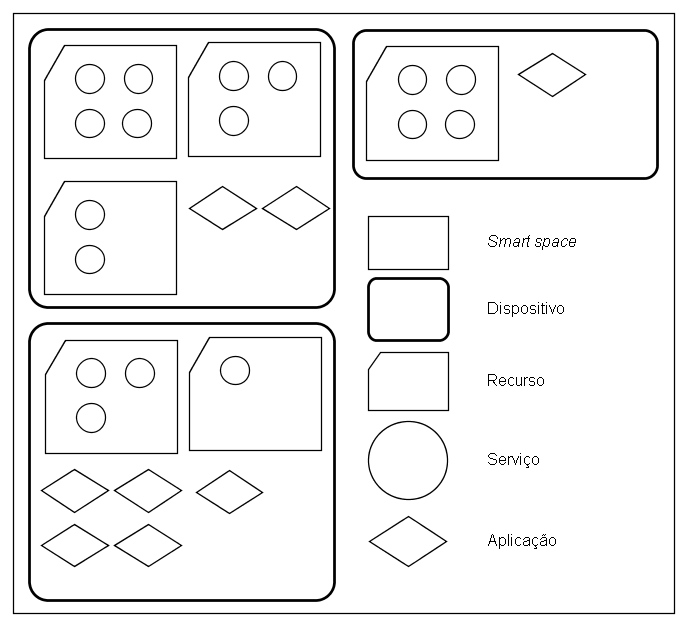
\includegraphics[scale=0.6]{imagens/arquiteturaDSOA}
	\caption{Exemplo da arquitetura DSOA.}
	\label{fig:arquiteturaDSOA}
\end{figure}

O \emph{uOS} possui a \emph{DSOA (Device Service Oriented Architecture)}, uma extensão da \emph{SOA (Service Oriented Architecure)}, como arquitetura. Como mostrado pela figura~\ref{fig:arquiteturaDSOA}, na DSOA podemos destacar cinco entidades básicas: ambiente inteligente, dispositivo, recurso, serviço e aplicações. O Ambiente inteligente é um espaço composto por pelo menos dois dispositivos com capacidade de computação conectados por meio de uma rede de comunicação colaborativa com os usuários. Um dispotivo é definido como um aparelho com capacidade de comunicação e que pode abrigar aplicações. Um recurso é definido como um grupo de funcionalidades relacionadas que podem ser acessadas por meio de interfaces pré-definidas. É a entidade básica de interação entre dispositivos. Um serviço é a implementação de uma funcionalidade disponibilizada pelo recurso para o ambiente com uma interface conhecida. As aplicações conferem inteligência ao ambiente executando nos dispositivos existentes e, a partir de informações providas pelos recursos conhecidos, podem realizar ações. 

Cada um dos conceitos apresentados na DSOA possui uma representação no \emph{uP} com seus respectivos atributos:

\begin{itemize}
	\item Dispositivo(\emph{UpDevice}):
	
		Por meio dos seguintes atributos, é possível identificar unicamente o dispositivo no ambiente, e quais são as interfaces rede que o dispositivo possui para realizar alguma comunicação:
		\begin{itemize}
			\item \emph{``name''}: 
			
			Identificador do dispositivo;
			\item \emph{``networks''}: 

			Lista de interfaces de rede do dispositivo. Cada interface é composta pelo tipo de rede e endereço do dispositivo.
		\end{itemize}
	\item \emph{Driver}(\emph{UpDriver}): 

		Representa o conceito do Recurso definido na DSOA. Como um dispositivo pode ter várias instâncias de um recurso, cada instância é identificada unicamente dentro do dispositivo que contém este recurso. O \emph{driver} é composto por:
		\begin{itemize}
			\item \emph{``name''}:

				Identificador do recurso no ambiente;
			\item \emph{``services''}:
				
				Lista de serviços síncronos do recurso;
			\item \emph{``events''}:
				
				Lista de serviços assíncronos do recurso.
		\end{itemize}
	\item Serviço(\emph{UpService}): 

		Representa o conceito de mesmo nome definido na DSOA. Sua interface é composta pelos seguintes atributos:
		\begin{itemize}
			\item \emph{``name''}:

				Identificador do serviço disponível no recurso;
			\item \emph{``parameters''}:
				
				Lista de parâmetros necessários para que o serviço seja executado. Esses parâmetros podem ser de dois tipos:
				\begin{enumerate}
					\item Opcional (\emph{OPTIONAL});
					\item Obrigatório (\emph{MANDATORY}).
				\end{enumerate}
		\end{itemize}
\end{itemize}

Segundo a DSOA, cada recurso, modelado na forma de um \emph{driver}, é identificado por um nome e não há qualquer tipo de relacionamento entre outros recursos. A \emph{DSOA} não define tipos básicos de recursos.	